\section{Visualizzazione}

\subsection{Terreno}

\subsection{Data Collection}\label{sec:data-col}

Dal momento che uno dei principali obiettivi della modellazione basata su agenti è la generazione di dati per l'analisi, Mesa offre una classe in grado di gestire la raccolta e l'archiviazione dei dati in modo tale da facilitarne l'analisi. Il \textbf{data collector} di Mesa consente di archiviare tre tipi di dati:

\begin{itemize}
    \item Variabili a livello di agente.
    \item Variabili a livello di modello.
    \item Tabelle di vario genere.
\end{itemize}

Le variabili a livello di agente e di modello vengono aggiunte al \textbf{data collector} insieme ad una funzione per raccoglierle. Queste ultime, nel caso di raccolta di dati del modello accettano come parametro il modello stesso, mentre quelle che raccolgono dati relativi agli agenti accettano in input il parametro rappresentante un agente.

Le funzioni utilizzate nello scenario di interesse sono a livello di modello e al momento della raccolta da parte del \textbf{data collector} i dati vengono aggregati in un dizionario, associando al valore dello step corrente il valore prodotto dalle funzioni di aggregazione.

I dati calcolati e raccolti dal \textbf{data collector} ad ogni step del modello sono i seguenti:

\begin{itemize}
    \item Numero totale di agenti: conta tutti gli agenti presenti all'interno del supermercato.
    \item Numero di agenti che stanno facendo la spesa.
    \item Numero di clienti che stanno effettuando il pagamento.
    \item Numero totale di agenti in coda.
    \item Numero medio di agenti in coda: questa misura aggregata viene calcolata tenendo conto di quello che è il numero di casse aperte in ogni istante temporale.
    \item Tempo medio trascorso in coda: questo parametro calcola il tempo medio di attesa in coda delle persone attualmente presenti nello scenario.
\end{itemize}

Questi dati sono stati poi utilizzati a fini di analisi e comparazione tra le diverse strategie di coda, andando a realizzare grafici che mostrano l'andamento di queste variabili in funzione del numero di step.

\subsection{Terreno}
Motivazione scelta grafica

\subsubsection{Tileset}
Un tileset è un'immagine suddivisa in celle (tile) quadrate aventi la stessa dimensione. Durante la progettazione della mappa è quindi possibile combinare in svariati modi tali celle per realizzare terreni complessi.

% https://www.spriters-resource.com/game_boy_advance/pokemonemerald/
La realizzazione grafica del progetto è basata sugli ambienti di Pokemon e, qualora necessario, si è intervenuti manualmente per personalizzare le celle. In [ref] viene riportato il tileset finale realizzato.

\begin{figure}[H]
    \makebox[\textwidth][c]{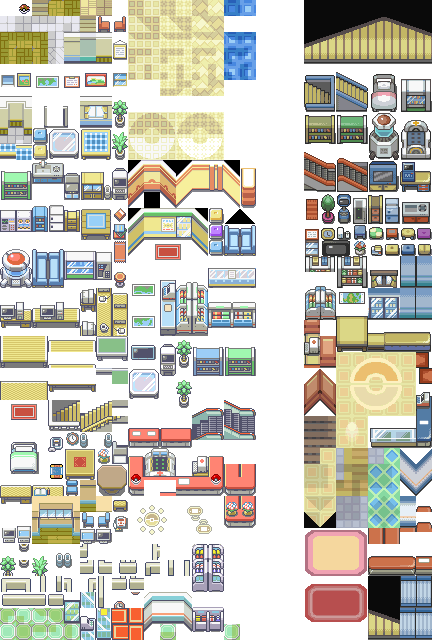
\includegraphics[width=0.8\linewidth]{tileset.png}}
    \caption{Tileset utilizzato con suddivisione in griglia}
    \label{fig:tileset}
\end{figure}

Le mappe sono state studiate appositamente ponendo particolare attenzione alle proporzioni degli ambienti e agevolate nella loro realizzazione con l'ausilio di un software apposito.

\subsubsection{TILED}
Tiled è un software open-source studiato per la costruzione di livelli focalizzato sulla semplicità di utilizzo.[cite:https://www.mapeditor.org/]
Questo ci ha permesso di creare rapidamente delle mappe ed apportare modifiche in corso d'opera efficientemente per poi esportare il lavoro realizzato in un formato utile alla successiva visualizzazione.

\subsubsection{Visualizzazione}
La lettura e la visualizzazione del terreno sulla griglia nativa di Mesa ha comportato modifiche sostanziali in alcuni file del framework.
In aggiunta, sono state applicate alcune ottimizzazioni per ridurre la complessità del processo di aggiornamento della griglia ad ogni step.
